%%%%%%%%%%%%%%%%%%%%%%%%%%%%%%%%%%%%%%%%%%%%%%%%%%%%%%%%%%%%%%%%%%%%%%%%%%%%%%%%%%%%%%%%%
%%                                                                                     %%
%%                This file is part of the CAPH Compiler distribution                  %%
%%                            http:%/caph.univ-bpclermont.fr                           %%
%%                                                                                     %%
%%                                  Jocelyn SEROT                                      %%
%%                         Jocelyn.Serot@univ-bpclermont.fr                            %%
%%                                                                                     %%
%%         Copyright 2011-2018 Jocelyn SEROT.  All rights reserved.                    %%
%%  This file is distributed under the terms of the GNU Library General Public License %%
%%      with the special exception on linking described in file ..%LICENSE.            %%
%%                                                                                     %%
%%%%%%%%%%%%%%%%%%%%%%%%%%%%%%%%%%%%%%%%%%%%%%%%%%%%%%%%%%%%%%%%%%%%%%%%%%%%%%%%%%%%%%%%%

\chapter{Image processing}
\label{cha:lang-ip}

In this last chapter, we describe the use of the \caph language to implement a more ``realistic'' image
processing application.

\medskip
This application performs edge extraction on images using the
well-known Sobel filter.

An example of input and output image is given Fig.~\ref{fig:pcb-ex}.

\begin{figure}[h]
\centering
  \begin{tabular}[c]{cc}
  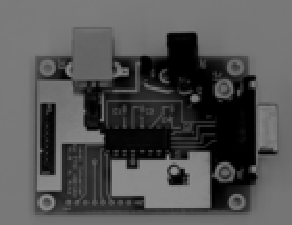
\includegraphics[width=0.2\textwidth]{figs/pcb.pdf} &
  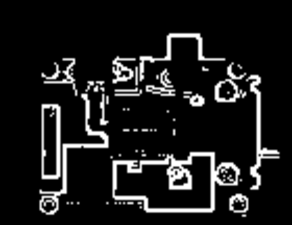
\includegraphics[width=0.2\textwidth]{figs/pcb-res.pdf} \\
  Input image & Result image
  \end{tabular}
  \caption{Edge extraction with the Sobel operator}
  \label{fig:pcb-ex}
\end{figure}

For each pixel $P_{i,j}$ of the input image, the magnitude of the local gradient is computed using
approximations of the horizontal and vertical derivatives $G_x$ and $G_y$, and the resulting value
is compared to a fixed threshold for producing a binary image (with edge pixels encoded as 1 and
background pixels as 0). To simplify, the magnitude of the gradient, $G=\sqrt{G_x^2+G_y^2}$, will be
here approximated as $|G_x|+|G_y|/2^n$, where $n$ is a scaling factor.

Considering we have three actors, \verb|grad|, \verb|asum|, \verb|thr|, computing respectively the
gradient components, the half sum their absolute values and the binarisation of an image, the dataflow
formulation of the corresponding is given in Listing~\ref{lst:sobel-1}.  Figure~\ref{fig:sobel-dot}
gives the corresponding dataflow network\footnote{The binarisation threshold has here been
  arbitrarily set to 20.}

\begin{figure}[htbp]
  \centering
 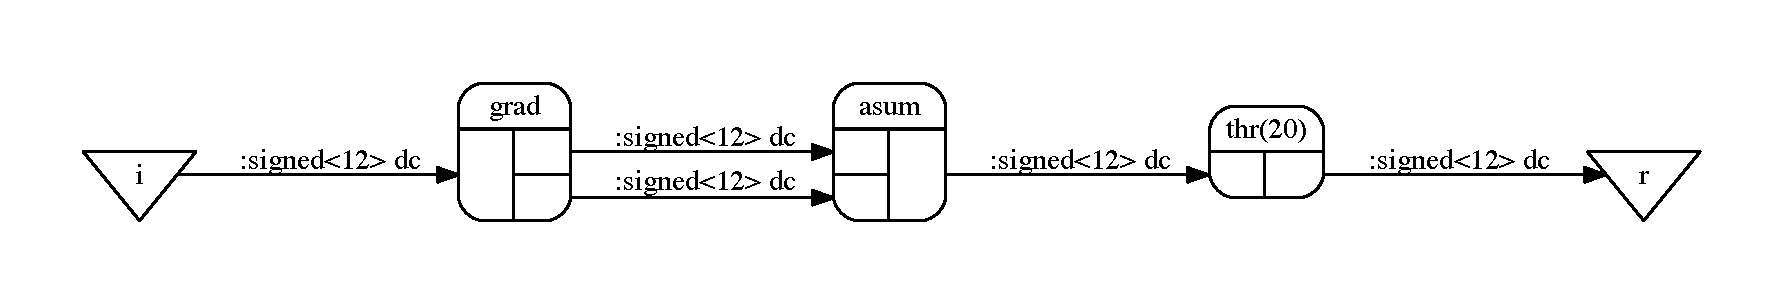
\includegraphics[width=0.9\textwidth]{./figs/sobel-dot.pdf}
  \caption{The graphical representation of the program given in Listing.~\ref{lst:sobel-full}}
  \label{fig:sobel-dot}
\end{figure}

\begin{lstlisting}[style=CaphStyle,numbers=left,numberstyle=\tiny,caption={A Sobel edge extraction
    application in Caph (top level description)},label={lst:sobel-1}]
actor grad in (i:signed<s> dc) out(o1:signed<s> dc, o2:signed<s> dc) ...
actor asum in ( i1:signed<s> dc, i2:signed<s> dc) out( o:signed<s> dc)  ...
actor thr (k:signed<s>) in ( i:signed<s> dc) out( o:unsigned<s> dc) ...

stream i:signed<12> dc from "pcb.txt";
stream r:signed<12> dc to "result.txt";

net (gx,gy) = grad i;         -- gradient x and y components
net gm = asum (gx, gy);       -- gradient magnitude (approx)
net r = thr 20 gm;
\end{lstlisting}

\medskip
The \verb|thr| actor is described in Listing~\ref{lst:sobel-thr}. This actor applies a binarisation
threshold to an image, returning a image of 1-bit unsigned pixels. The binarisation threshold is
specified as a parameter (\verb|t|, line 1), whose value will be set when instanciating the actor at
the network level (see line 10 in Listing.~\ref{lst:sobel-1}). Binarisation is performed by simply
comparing each pixel value to the threshold (last rule, line 7). 

\begin{lstlisting}[style=CaphStyle,numbers=left,numberstyle=\tiny,caption={The \texttt{thr} actor in
    Caph},label={lst:sobel-thr}]
actor thr (k:signed<s>)
  in ( i:signed<s> dc)
  out( o:unsigned<1> dc)
rules i -> o
| '< -> '<
| '> -> '>
| 'p -> if p>k then '1 else '0
;
\end{lstlisting}

\medskip The \verb|asum| actor is described in Listing~\ref{lst:sobel-magn}. This actor takes the
computes an approximation of the gradient magnitude by summing the absolute value of its two
components and dividing it by 2. The computation of the absolute value is
performed using the global function \verb|fabs|, which is declared before the actor.  The division
by 2 is implemented using the bit-shift builtin operator \verb|>>|.

\begin{lstlisting}[style=CaphStyle,numbers=left,numberstyle=\tiny,caption={The \texttt{asum} actor in
    Caph},label={lst:sobel-magn}]
function fabs x = if x < 0 then -x else x : signed<s> -> signed<s>;

actor asum
  in ( i1:signed<s> dc, i2:signed<s> dc)
  out( o:signed<s> dc)
rules (i1,i2) -> o
| ('<,'<) -> '<
| ('>,'>) -> '>
| ('p,'q) -> '(fabs(p)+fabs(q))>>1
;
\end{lstlisting}

\medskip
The computation of the gradient components could be carried out by writing out dedicated actors, in the
vein of those described in Sec.~2.5 of the reference manual. We will here adopt a more straightforward
approach and rely on the predefined convolution actors provided in the standard CAPH library. The
gradient $x$ and $y$ component can be computed by convolving the input image with the 2D kernels
showed in Fig.~\ref{fig:sobel-kernels}.

\begin{figure}[h]
\centering
  \begin{tabular}[c]{cc}
$ G_x = \begin{pmatrix}
      1 & 0 & -1 \\
      2 & 0 & -2 \\
      1 & 0 & -1 \\
    \end{pmatrix} $ &
$ G_y = \begin{pmatrix}
      1 & 2 & 1 \\
      0 & 0 & 0 \\
      1 & 2 & 1 \\
    \end{pmatrix} $
  \end{tabular}
  \caption{Convolution kernels for computing the gradient $x$ and $y$ components}
  \label{fig:sobel-kernels}
\end{figure}

For this, the file \verb|convol.cph| provides the actor \verb|conv233|. This actor accepts three
parameters~:
\begin{itemize}
\item a convolution kernel, given as a 2D array $k[0..2][0..2]$
\item a scaling factor $n$,
\item a padding value $v$.
\end{itemize}
Given a $M\times N$ input image $x$, represented as a structured stream 

\begin{center}
\begin{math}
<\ <\ x_{1,1}\ x_{1,2}\ ...\ x_{1,N}\ >\ <\ x_{2,1}\ x_{2,2}\ ...\ x_{2,N}\ >\ ...\ <\ x_{M,1}\ x_{M,2}\ ...\ x_{M,N}\ >\ >
\end{math}
\end{center}

\noindent
the \verb|conv233| actor computes an output image $y$, with the same representation and dimensions

\begin{center}
\begin{math}
<\ <\ y_{1,1}\ y_{1,2}\ ...\ y_{1,N}\ >\ <\ y_{2,1}\ y_{2,2}\ ...\ y_{2,N}\ >\ ...\ <\ y_{M,1}\ y_{M,2}\ ...\ y_{M,N}\ >\ >
\end{math}
\end{center}

\noindent
where 

\begin{equation}
y_{i,j} = 
\begin{cases}
v & \text{if}\ 1 \leq 2\ \text{or}\ 1 \leq j \leq 2 \\
\sum\limits_{\substack{0\leq i'\leq 2\\ 0\leq j'\leq 2\}}} k_{2-i',2-j'}.x_{i-i',j-j'}\quad /2^n & \text{if}\ 2\leq i\leq M\ \text{and}\ 2\leq j \leq N
\end{cases}
\label{eq:conv233}
\end{equation}

The corresponding formulation in CAPH is given in Listing~\ref{lst:sobel-conv}. The convolution
kernels $G_x$ and $G_y$ are specified as 2S arrays. The padding value $v$
(for the first two lines and columns) has here been set to 0 and the scaling factor is also 0.

\begin{lstlisting}[style=CaphStyle,numbers=left,numberstyle=\tiny,caption={Computation of the
    gradient components using the \texttt{conv233} actor of the standard CAPH library},label={lst:sobel-conv}]
net gx = conv233 ([[1,0,-1], [2,0,-2], [1,0,-1]], 0, 0) i;  -- grad x component
net gy = conv233 ([[1,2,1], [0,0,0], [-1,-2,-1]], 0, 0) i;  -- grad y component
\end{lstlisting}

\medskip
The complete source code of the application is given in
Listing~\ref{lst:sobel-full}\footnote{It can also be found in directory
  \texttt{examples/working/primer/sobel} of the distribution.}. The corresponding dataflow graph is
given in Fig.~\ref{fig:sobel-full}. To simplify further assessment, the name of the input file and
the binarisation threshold are here specified indirectly by using references to \emph{macros}.
The corresponding values will be set
when invoking the compiler (with the \verb|-D| option), thus
offering a way of changing them without having to edit the source file (see Sec.~9.9 of the manual).

\begin{lstlisting}[style=CaphStyle,numbers=left,caption={Complete source code of the Sobel-based
    edge extraction},label={lst:sobel-full}]
#include "convol.cph"

function fabs x = if x < 0 then -x else x : signed<s> -> signed<s>;

actor asum
  in ( i1:signed<s> dc, i2:signed<s> dc)
  out( o:signed<s> dc)
rules (i1,i2) -> o
| ('<,'<) -> '<
| ('>,'>) -> '>
| ('p,'q) -> '(fabs(p)+fabs(q))>>1
;

actor thr (k:signed<s>)
  in ( i:signed<s> dc)
  out( o:unsigned<1> dc)
rules i -> o
| '< -> '<
| '> -> '>
| 'p -> if p>k then '1 else '0
;

stream i:signed<12> dc from %ifile;
stream r:unsigned<1> dc to "result.txt";

net gx = conv233 ([[1,0,-1],
                   [2,0,-2],
                   [1,0,-1]],0,0) i;    -- grad x component
net gy = conv233 ([[1,2,1],
                   [0,0,0],
                   [-1,-2,-1]],0,0) i;  -- grad y component
net gm = asum (gx, gy);                 -- grad amplitude (approx)
net r = thr %threshold gm;
\end{lstlisting}

\begin{figure}[htbp]
  \centering
 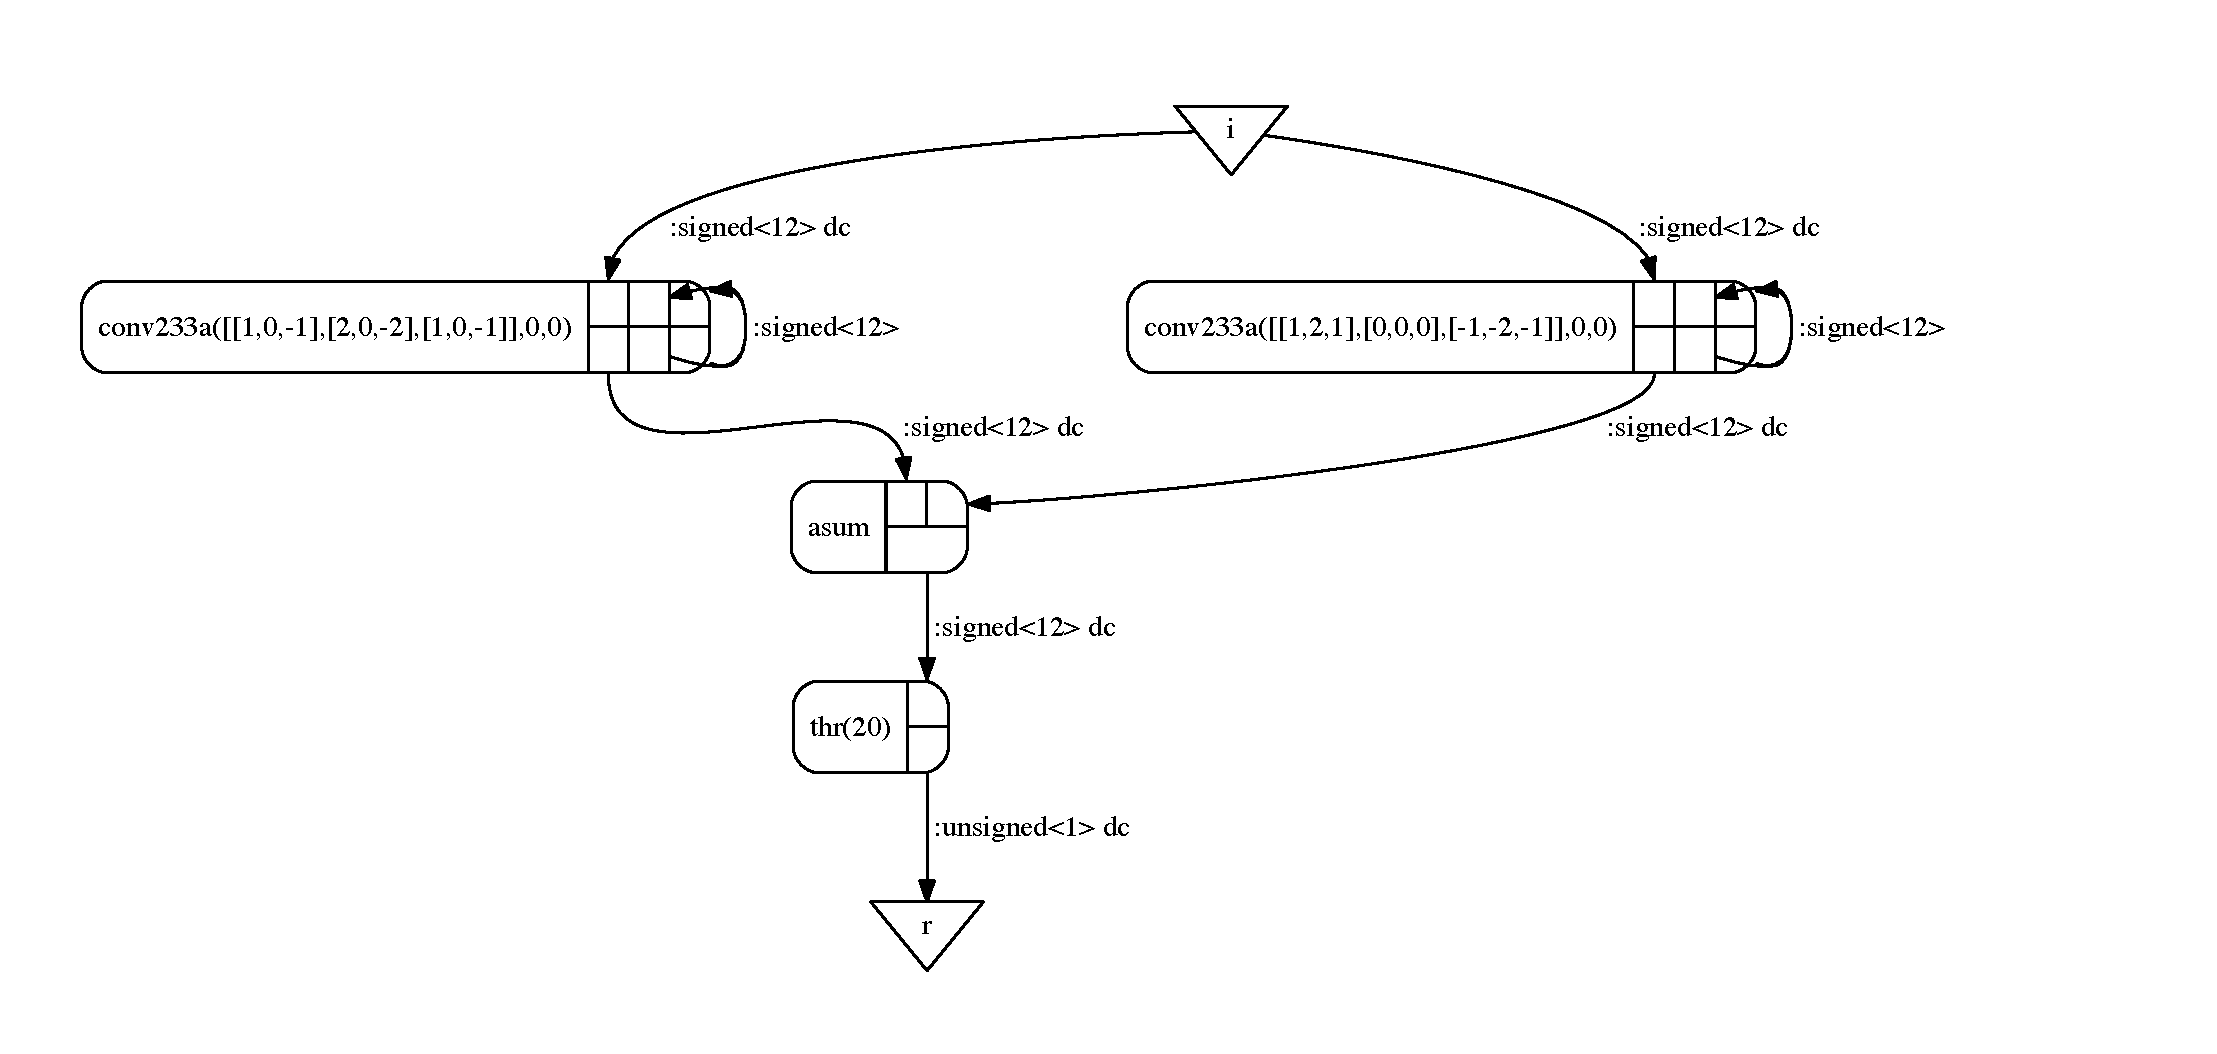
\includegraphics[width=\textwidth]{./figs/sobel-full.pdf}
  \caption{The graphical representation of the program given in Listing.~\ref{lst:sobel-full}}
  \label{fig:sobel-full}
\end{figure}

\bigskip
As for the application of the previous chapter, we will describe the implementation, simulation and
synthesis of this application in part 3 of this document.

%%% Local Variables: 
%%% mode: latex
%%% TeX-master: "caph-primer"
%%% End: 
